

\tikzset{every picture/.style={line width=0.45pt}} %set default line width to 0.75pt   

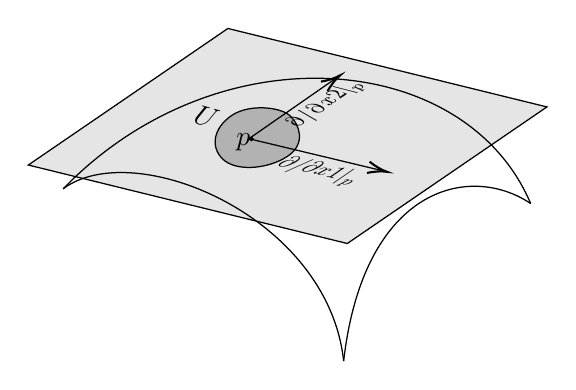
\begin{tikzpicture}[scale=0.85, x=0.75pt,y=0.75pt,yscale=-1,xscale=1]
%uncomment if require: \path (0,360); %set diagram left start at 0, and has height of 360

%Shape: Rectangle [id:dp08691604933838892] 
\draw  [fill={rgb, 255:red, 229; green, 229; blue, 229 }  ,fill opacity=1 ] (193.4,31.09) -- (374.22,75.57) -- (261.08,152.98) -- (80.26,108.5) -- cycle ;
%Shape: Polygon Curved [id:ds13972230036871047] 
\draw  [fill={rgb, 255:red, 178; green, 178; blue, 178 }  ,fill opacity=1 ] (195.67,80.33) .. controls (205.67,73.67) and (223,75.67) .. (228.33,80.33) .. controls (233.67,85) and (238.33,96.33) .. (227,103.67) .. controls (215.67,111) and (197.67,112.33) .. (190.33,105) .. controls (183,97.67) and (185.67,87) .. (195.67,80.33) -- cycle ;
%Curve Lines [id:da3913670271390508] 
\draw    (100,122) .. controls (140,92) and (250.33,137.67) .. (259,219.67) ;
%Curve Lines [id:da7387351338025494] 
\draw    (100,122) .. controls (188.33,31) and (328.33,43.67) .. (365,130.33) ;
%Curve Lines [id:da8758985242679558] 
\draw    (259,219.67) .. controls (270.33,121) and (330.33,107) .. (365,130.33) ;
%Shape: Circle [id:dp9796756156419224] 
\draw  [fill={rgb, 255:red, 0; green, 0; blue, 0 }  ,fill opacity=1 ] (205.67,93.67) .. controls (205.67,93.11) and (206.11,92.67) .. (206.67,92.67) .. controls (207.22,92.67) and (207.67,93.11) .. (207.67,93.67) .. controls (207.67,94.22) and (207.22,94.67) .. (206.67,94.67) .. controls (206.11,94.67) and (205.67,94.22) .. (205.67,93.67) -- cycle ;
%Straight Lines [id:da8885224032682308] 
\draw    (204.99,93.82) -- (255.36,58.81) ;
\draw [shift={(257,57.67)}, rotate = 145.2] [color={rgb, 255:red, 0; green, 0; blue, 0 }  ][line width=0.75]    (10.93,-3.29) .. controls (6.95,-1.4) and (3.31,-0.3) .. (0,0) .. controls (3.31,0.3) and (6.95,1.4) .. (10.93,3.29)   ;
%Straight Lines [id:da022213529301427393] 
\draw    (205.67,93.67) -- (281.67,111.88) ;
\draw [shift={(283.61,112.35)}, rotate = 193.48] [color={rgb, 255:red, 0; green, 0; blue, 0 }  ][line width=0.75]    (10.93,-3.29) .. controls (6.95,-1.4) and (3.31,-0.3) .. (0,0) .. controls (3.31,0.3) and (6.95,1.4) .. (10.93,3.29)   ;

% Text Node
\draw (196.67,89.4) node [anchor=north west][inner sep=0.75pt]    {$p$};
% Text Node
\draw (177.02,73.02) node [anchor=north west][inner sep=0.75pt]  [rotate=-15.82,xslant=0.18]  {$U$};
% Text Node
\draw (229.85,100.72) node [anchor=north west][inner sep=0.75pt]  [font=\scriptsize,rotate=-13.8,xslant=0.89]  {$\partial /\partial \sub x{1} |_{p}$};
% Text Node
\draw (219.33,84.95) node [anchor=north west][inner sep=0.75pt]  [font=\scriptsize,rotate=-326.11,xslant=-0.89]  {$\partial /\partial \sub x{2} |_{p}$};


\end{tikzpicture}
